%\documentclass[11pt]{article}
\documentclass[print,ms]{nuthesis}
%\usepackage{times}

%\setlength{\textwidth}{6.5in}
%\setlength{\textheight}{9.0in}
%\setlength{\topmargin}{-.5in}
%\setlength{\oddsidemargin}{-.0600in}
%\setlength{\evensidemargin}{.0625in}

\newcommand{\secref}[1]{Section~\ref{#1}}
\usepackage{xcolor}

\usepackage[dvipdfm,%
bookmarks=true,%
bookmarksopen=true,%
bookmarksnumbered=true,%
bookmarkstype=toc,%
pdftitle={Derek Weitzel Thesis - Campus Grids},%
pdfsubject={},%
pdfauthor={Derek Weitzel},%
pdfkeywords={Weitzel, Grid, Campus},
%linktocpage=true,
linkbordercolor=white
]{hyperref}


%\newcommand{\doublespace}{\baselineskip0.34truein}
%\newcommand{\singlespace}{\baselineskip0.16truein}
%\newcommand{\midspace}{\baselineskip0.24truein}
%\newcommand{\midplusspace}{\baselineskip0.26truein}




%\usepackage{setspace}
\usepackage{algorithmic}
\usepackage{algorithm}

\usepackage{graphicx}
\usepackage{calc}
\usepackage{url}
\usepackage{listings}
\usepackage{subfig}

\newlength{\imgwidth}

\newcommand\scalegraphics[1]{%   
    \settowidth{\imgwidth}{\includegraphics{#1}}%
    \setlength{\imgwidth}{\minof{\imgwidth}{\textwidth}}%
    \includegraphics[width=\imgwidth]{#1}%
}



%\doublespacing

%\author{Derek Weitzel\\
%Computer Science and Engineering\\
%University of Nebraska--Lincoln\\
%Lincoln, NE 66588-0115\\
%dweitzel@cse.unl.edu
%       }
       
\begin{document}
\frontmatter
\title{Campus Grids}
\author{Derek Weitzel}
\adviser{Dr. David Swanson}
\adviserAbstract{Dr. David Swanson}
\major{Computer Engineering}
\degreemonth{May}
\degreeyear{2011}

\maketitle

\begin{abstract}

It is common at research institutions to maintain multiple clusters.  These might fullfill different needs, different policies, or  represent generations of hardware.  Many of these clusters are under utilized while researchers at other departments may require these resources.  Linking these clusters with traditional grid software would require changes in security and execution environments.  In this paper we will describe a framework and technology that are used to link departmental clusters such that submission at one cluster could lead to execution on another.  We evaluate the framework on five important attributes found in campus grids.  This framework is then further expanded to bridge campus grids into a regional grid.

%the framework is designed as lightweight, and leveraging existing security infrastructure.   All of these components are functional and are running research jobs in production.

\end{abstract}

%\newpage
\tableofcontents
%\newpage

% \doublespace
\mainmatter
\chapter{Introduction}
\label{sec:Introduction}

%\subsubsection* {The problem we have solved}

%\begin{itemize}
%\item
%Concentrate on making {\em this} assertion and {\em only} this assertion in a
%succinct set of 1 to 3 paragraphs 

%\item Department clusters waste power by being under utilized for significant portions of time.
%\item Researchers have peaks in usage and need overflow capacity.
%\item Move single core jobs around to idle clusters, freeing up space for MPI jobs.
%\item Users want a single execution environment.  This is an expressed goal of the Condor project.
%\item Increased utilization of a cluster can reflect well on the department.
%\item Use existing security infrastructure.

%\item
%A common mistake is to explain too much of the problem context first. Instead,
%state the problem essentially as a claim, and leave explanations supporting
%your claim to the next part, ``Why it is not already solved.''

%\end{itemize}

A campus grid is a framework for distributing computation among independent clusters within a campus.  A campus typically consists of multiple compute clusters that are independently administered.  A campus grid's purpose is to increase the processing power accessible to users by connecting compute resources.   The compute clusters can benefit from increased utilization, while the users can benefit by increased processing power.  

The Holland Computing Center (HCC) created a campus grid that spans two clusters and can overflow onto national grid infrastructure.  The HCC grid borrowed concepts and techniques from earlier campus grids and a national grid.  The campus grid is quickly becoming the model of a homogeneous campus grid at other sites.

The HCC campus grid bridges clusters and the national infrastructure while running production processing jobs from on-campus researchers. Over the last X (TODO find stats on number of hours) we have ran Y hours on the campus grid, along with Z hours bridging to other campus grids.


Generally, users are provided a uniform interface to submit jobs to remote clusters inside their campus.  In many campus grids, the user manually submits to specific clusters.  In others, a layer of software distributes the computation among clusters in the grid. 

Building a campus grid represents a significant commitment for both users and resource providers, which should be 
evaluated against the benefits.  The primary benefits are:
\begin{itemize}
\item \textbf{Resource sharing}: An HTC-based approach focusses on using all resources effectively.  Resources are 
typically bought for peak, not average, usage; integrating the idle time across the entire campus and using it improves 
the value of the investment.
\item \textbf{Homogeneous interfaces to multiple resources}: Moving researchers from one resource to another results in 
a (possibly large) upfront cost in time and energy.  By providing a homogeneous interface across the campus, 
researchers can quickly utilize new resources without the pain of migration.
\item \textbf{Independence from any single computational resource}:  It is expensive to provide highly available 
resources.  If do not rely on a specific single cluster, individual cluster downtimes have a smaller impact.  This 
reduces the need for high levels of redundancy and stretches the campus computing budget further.
\end{itemize}

An obvious requirement for campus grids is having multiple resources on campus.  However, this is not sufficient for 
resource providers - the resources should also be interchangeable.  A grid composed of a single AIX cluster, Linux 
cluster, and Windows cluster, will likely never see any resource pooling or sharing.  This does not necessarily imply 
the resources need to be identical - complete homogeneity is typically impossible due to individual resource 
requirements or ownership.

A mistake in campus grids is to focus on the infrastructure for pooling resources without similarly engaging and 
supporting the activities of users.  An analogy can be made to flows: if there is a sink (resources) with no source 
(user jobs), the flow quickly stops, and the campus grid is forgotten.  Personnel investment must be made to engage 
the user community.  Even before this investment is made, a campus should identify whether the on-campus scientific 
computing has a significant portion of tasks that can be converted to HTC workflows.  Prioritization should be applied 
so the users with the simplest workflow and the most to benefit are converted first.  Tasks with the following 
characteristics should typically be avoided:

\begin{itemize}
\item Large scale (multi-node) MPI, as these require specific tunings to the given resource.
\item Multi-day jobs.  Shared resources often need to be reallocated quickly back to the owner, meaning these jobs are 
unlikely to complete.
\item Sensitive data or software.  Tasks with sensitive (for example, HIPPA-protected) data may have legal boundaries 
preventing distribution.  Software with strict licenses may also be illegal to use across the grid.
\end{itemize}

An common advantage for using campus grids is to alleviate demand on newer parallel machines by moving single core jobs to other clusters that have idle cycles.  Recently, the single core performance has been stagnant, therefore moving the single core jobs to the older hardware will not significantly decrease performance.  Also, by moving the single core jobs, it can free the newest hardware for large parallel jobs which can benefit from better interconnects, larger and faster storage, and increased core count that are on the newest hardware.


%As the speed of innovation in computing increases, it is common for a campus to have multiple generations of clusters.  These clusters are commonly bought as independent systems, not meant to share work between them.  This causes users to flock to the newest generation hardware, hoping to increase the performance of their application.  This movement of users leads to under utilization of older hardware, and increased demand on the newest.

%This is just one of many situations that would cause users to underutilize hardware.  Other situations could be:

%\begin{itemize}
%\item \textbf{Departmental clusters:}  Each department has a dedicated cluster.  This cluster specialization can cause under utilization when department researchers are not using the resources.
%\item \textbf{Peaks of usage:} In general, users have peaks to their usage around deadlines.
%\item \textbf{Parallel jobs:} While a cluster is draining nodes for a large parallel job, the cluster could fill those drained slots with pre-emptable usage.
%\end{itemize}

One way to alleviate this demand is to move single core jobs to other clusters that have idle cycles.  Recently, the single core performance has been stagnant, therefore moving the single core jobs to the older hardware will not significantly decrease performance.  Also, by moving the single core jobs, it can free the newest hardware for large parallel jobs which can benefit from better interconnects, larger and faster storage, and increased core count that are on the newest hardware.




%\subsubsection* {Why the problem is not already solved or other solutions 
%are ineffective in one or more important ways}


%\item
%Your new idea need not solve every problem but it should solve at least one
%that is not already solved

There have been several attempts to create a distributed campus grid.  They all use some technology to distribute and schedule the jobs on the grid.  Some methods for distribution are commercial products such as Moab \cite{website:moabgrid}.  Others are translation layers between a generic description language and a scheduler, such as Globus \cite{foster1997globus}.  Still others are entire resource managers that can span multiple clusters like Condor \cite{thain2005distributed}.  Each of these solutions can be built to create a campus grid, but they all have drawbacks that are highlighted below.






%\item 
%A common solution to linking clusters is condor flocking.  Flocking requires every cluster to run condor daemons on their nodes.  

% Last case, since it's simalar to mine.
%Several universities have approached the problem utilizing condor flocking.

%\item
%This is the place to provide a succinct description of the problem context
%giving enough information to support the claim that a problem exists, made in
%the preceding problem declaration.





%\subsubsection* {Why our solution is worth considering and why is it effective
%in some way that others are not}

The framework described in this paper creates a production campus grid.  The campus grid includes technology to allow clusters to join the campus grid.  It integrates clusters that use several schedulers, and uses production quality software integrated into a solution that is deployed at several cluster in the U.S.

The campus grid framework provides a method for users to run jobs transparently on distributed resources.  The jobs are sent to available resources on distributed clusters on the campus grid.  Further, it can expand beyond the campus and onto other campuses by simple configuration changes.

The campus grid is used in production at the University of Nebraska, connecting two geographically separate clusters.  Users utilize the campus grid by submitting to one connected clusters, while their jobs run on either cluster.  The jobs are transported with their input files to a execution sandbox on the worker node.  Further, the campus grid expands beyond Nebraska, reaching Purdue and Clemson university.


% This will largely be from CHEP paper
\section{Attributes of Campus Grids} \label{sec:attributes}
In this section, we explore five characteristics of HTC-centric campus grids. While the list isn't exhaustive, we've 
found campus grids can be characterized by how they approach trust relationships, job submission, resource 
independence, accounting, and data management.


\subsection{Trust relationships}
A successful campus grid must have an acceptable trust model in order to succeed.  A trust relationship enables 
a resource provider to grant campus users controlled access to the resource, and may be established through 
 sociology and/or technology-based security methods.

In the OSG, the trust model used is designed to be homogeneous and to meet the most stringent requirements of 
all participating sites.  The implementation involves using Globus's Grid Security Infrastructure (GSI) with VOMS 
attributes a PKI extension \cite{farrell2002rfc3281}.  The GSI model is widely 
accepted, allowing the OSG to participate in the Worldwide LHC Computing Grid (WLCG).  Fermigrid's campus grid user 
authentication is based on the GSI model.  While it provides a highly secure, decentralized authorization model and 
proven at the worldwide scale, it is more difficult for end users compared to traditional username/password 
authentication.  Thus, campus grids may be motivated to use alternate trust models.

On-campus resource providers may have a higher degree of trust than at the national level due to 
sociological reasons.  This trust may just be based on locality -- it is easier to establish a working relationship 
with a colleague locally on campus than 1000 miles away.

A technical reason for different trust relationships between campuses and larger grids is the location of user 
job submit hosts.  Unlike the OSG, where users can submit jobs from any worldwide host, campus users often submit from 
a few trusted campus resources.  If limited to a few well-managed hosts, IP-based security may be sufficient for 
campuses, as the security is applied to submit hosts rather than cluster entry points.

Security requirements on some university campuses are simply less stringent than that of federal labs, explaining 
Purdue and Wisconsin's preference for IP security compared to FermiGrid's GSI.  A campus may 
not have strict policies governing user job separation or traceability requirements.  Some campus clusters may be 
satisfied with running any job originating from elsewhere on the campus to an unprivileged account.  When a job crosses 
domains (from local cluster to across campus, or from campus to the national grid), it must 
satisfy the security requirements for the destination domain.  Thus, if a campus grid would like to bridge to the 
national grid, users most be able to associate GSI credentials with their jobs.


\subsection{Job submission}
In order for a HTC-oriented campus grid to function, users need a usable job submission interface.
The Globus Toolkit \cite{foster1997globus} provides the GRAM interface for job 
submission and corresponding clients.  GRAM layer abstracts above the batch system; the 
user interacts with GRAM, and GRAM converts these actions into batch system commands at the destination.
The GRAM interface is used by the OSG, and is being used at the scale of over 100 million jobs a year.  The GRAM 
interface abstracts many batch system constructs, and is also used 
on the TeraGrid to submit larger jobs running on hundreds or thousands of cores.  While GRAM can be used directly, 
users almost exclusively prefer to interact with it via Condor-G  \cite{frey2002condor} , which provides a batch 
system interface on top of GRAM.  Fermigrid relies on Condor-G submission to GRAM for job submission.

An abstraction layer like GRAM introduces a new user experience (even if Condor-G is used), requiring new expertise. An 
alternate approach is to use batch system software that can interact with multiple instances of itself.  By 
linking resources at the batch system level rather than adding an abstraction layer on top, we improve the user 
experience - users no longer need to learn additional tools.  The tools do not need to translate errors across 
different domains, easing a common source of frustration in the grid.  When Condor-G is used, we have a batch-system 
interface abstracting an API which, in turn, abstracts remote batch systems - error propagation is extremely difficult.  
In the Purdue, GLOW, and HCC campus grids, 
resources are linked through use of a common batch system, Condor, through a mechanism Condor refers to as 
``flocking".  A hybrid between Condor-only and GRAM is given by GlideinWMS \cite{sfiligoi2008making}.

In our observations, the closer the grid user experience is to the batch system user experience, the more likely a 
user will adopt the campus grid.



\subsection{Resource Independence}
Compared to a corporate IT environment, one unique aspect of universities is the diversity of management of 
computing 
resources.  On a campus, several distinct teams may manage distinct clusters due to campus 
organization or ownership.  Management of resources may be divided by college or departmental level.  One 
characteristic of campus grids is thus the independence of resources - the level of decision-making delegated out to 
the resource providers.

The simplest campus grids can be formed by requiring all clusters on campus to run the same batch system and linking 
batch system instances - GLOW's use of Condor is an example.  Every cluster in GLOW runs the Condor batch system, 
providing a common interface.  System administrators are not free to chose their own batch systems if they want to 
participate in this grid (participation is voluntary, and participants obviously believe the benefits of GLOW 
membership outweighs this drawback).  It may be desirable for a specialized cluster to have a distinct batch system  
from the rest of the campus; resource independence allows the cluster owners to best optimize their resource to suit 
their needs.

Resource independence comes at a cost to the end-user.  Extremely heterogeneous resources can be difficult to 
integrate at the software level - a binary compiled for Linux will not be compatible with Windows.  Some guarantees 
about the runtime environment or other interfaces need to be clearly articulated to prevent frustration.  Differences 
that are unavoidable or are expected to be handled by the user should be clearly expressed to the user \cite
{raman2002matchmaking}.  At the OSG level, we have found the users often frustrated by the amount of heterogeneity, 
especially compared to using a single site or a grid with a smaller number of sites \cite{zvada2010cdf}.


\subsection{Accounting}
Accounting may not seem to be an important grid characteristic -- it certainly isn't required for 
users to successfully run job.  However, it is critical for the long term health as it provides a quantitative 
measurement of the grid's value.  Accounting is also required for resource and users to ``barter" computing hours, one  
economic model for the grid.

Accounting systems do not need to be technically advanced.  Most batch systems provide a local accounting 
system.  The most basic method is for each cluster to parse these logs into a CSV file per cluster, and to 
build an Excel spreadsheet out of the aggregated files.  This is functional, but painful when statistics are needed 
more than once a month.  Most batch system vendors sell accounting systems usable for multiple clusters, provided all 
clusters involved use the same batch system.

Many research computing centers have written their own accounting systems at some point; most implementations are in 
the style of  PHP-based web interface on top of a custom database, again fed by custom log-parsing scripts. Both the 
OSG and TeraGrid have spent effort on accounting software to suite their needs.  The OSG�s, Gratia \cite{gratiaweb}, is 
designed to be reusable by other organizations, and is in use by all four campus grids�discussed in this paper.

Any site-local accounting systems -- homegrown, vendor provided, or designed for the national 
grids -- can work at the campus grid level as long as they can answer the following questions for a given time 
period:
\begin{itemize}
\item How much computing resource was consumed overall?
\item How much computing resource did a specific user/group consume?
\item How much computing resource did a specific user/group consume on resources they did not own? I.e., 
�How much did I get from resource sharing?�
\item How much computing resource did a specific cluster provide?
\item How much computing resource did a specific cluster provide to groups that did not own it?  I.e., �How 
much did I give away due to resource sharing?�
\end{itemize}




\subsection{Data Management}
Scientific data management presents two challenges for research computing centers: volume of data and archival 
requirements.  The data volume is often larger than a single scientist can keep on his personal systems, and 
archiving requires expertise outside his field.

Distributed computing can present an additional challenge: managing data location.  Data access costs may be 
variable between different resources on a grid, or required data may simply be unavailable at some locations.  A simple 
solution is to export the same file system to all resources, hiding data locality from the user.  Unfortunately, this 
solution breaks down outside the campus and may break down in highly-distributed campuses.

More complex solutions include declaring data dependencies for jobs explicitly inside the job 
submissions (gLite WMS \cite{andreetto2008glite}, Condor), promoting data to be a top-level abstraction like jobs (Stork \cite
{kosar2005stork}), or promoting data to be the central concept instead of jobs (iRODS \cite{irodswebsite, 
rajasekar2007irods}).  The CMS model separates the data management and job submissions systems, allowing the job 
submissions to simply assume all data is available (CMS PhEDEx \cite{phedex}).

While any system can be used for campus grids, the examples we consider in Sections \ref{sec:others} and \ref
{sec:hcc} either export a file system or utilize the tools from the job submission system.  The addition of a separate 
data management system often presents such complexity to the users that not buying more hardware and not using 
distributed computing is the cheaper alternative.  However, we note iRODS is an increasingly popular option and may 
have significantly decreased the operational cost of data management systems.


\section{Background}
\subsection{High Throughput Computing}
High Throughput Computing (HTC) is defined as tasks that require as much computing power (throughput) as possible over long periods of time \cite{gridbook-htc}.  This is in contrast to High Performance Computing (HPC), where users are concerned with response time.  This style is typified by ensembles of independent single processor jobs with no communication between them.  This is not to say there isn't coordination, many workflow managers can utilize HTC to solve complex problems with many steps.  

As there is no parallel communication between the jobs in a given task, they can be distributed across multiple resources.  This increases 
throughput, the end-goal of HTC.  HTC can use pooled resources mostly interchangeably and as such is well suited to 
distributed and grid computing models.  The OSG has demonstrated its technologies are successful; in Q4 2010, the OSG 
averaged over a 400,000 jobs and a million computational hours a day using HTC.


\subsection{Condor}
Condor is a high--throughput batch computing system developed at the University of Wisconsin - Madison.  An overview from \cite{thain2005distributed}:
\begin{quotation}
Condor is a high-throughput distributed batch computing system.  Like other batch systems, Condor provides a job management mechanism, scheduling policy, priority scheme, resource monitoring, and resource management.  Users submit their jobs to Condor, and Condor subsequently chooses when and where to run them based upon a policy, monitors their progress, and ultimately informs the suer upon completion.  
\end{quotation}

An important technology used in Condor is the ClassAd mechanism.  ClassAds are the language that Condor uses to communicate between daemons.  A ClassAd is a list of keys and values, where the values can be strings, numbers, or expressions.  All resources are described by ClassAds.  Job ClassAds have attributes such as log file, output, input, and job requirements.  Resource ClassAds have requirements to run on the resource, ownership, and policies.  ClassAds are used for matching jobs to resources by evaluating requirements of both the jobs and the resources.

Another component of Condor is the grid computing agent Condor-G \cite{frey2002condor}.  Condor-G communicates with Globus \cite{foster1997globus} sites.  Condor provides job submission, error recovery, and creation of a minimal execution environment.  Along with Condor-G, Condor can also submit jobs to other systems including Amazon EC2 \cite{amazonec2} and PBS \cite{pbstorque}.

\subsection{Open Science Grid}
The Open Science Grid (OSG) \cite{pordes2007open} is a national cyber infrastructure consortium that provides dedicated and opportunistic use of computation and storage resources.  The OSG consists of nationally distributed universities and national laboratories that provide access to shared computing and storage.  The OSG provides infrastructure, software, and engagement to the users.  

The OSG provides a common interface to computing and storage resources: Globus and SRM/GridFTP respectively.  Clients can access the resources by a OSG provided client.  Both Globus and SRM/GridFTP where developed by consortium members and included into the OSG packaging.  Many software modules have been contributed to the OSG software stack such as Condor and the Berkeley Storage Manager \cite{Bestman}.




% Do we need this?  Probably not, this is what the paper is about.
%\subsection{Campus Grids}






%\begin{itemize}
%\item
%A succinct statement of {\em why} the reader should care enough to read the
%rest of the paper.
%\item The framework described in this paper is designed as a modular framework that will allow clusters to overflow onto each other and to the grid.  This framework requires running condor on only one node in the cluster.  Each job that comes from another cluster will go through the default scheduler, whether it's PBS, SGE, or LSF.

%\item
%This should include a statement about the characteristics of your solution to
%the problem which 1) make it a solution, and 2) make it superior to other
%solutions to the same problem.

%\end{itemize}


%\subsubsection* {How the rest of the paper is structured}


\section{Paper Overview}
The rest of this paper first discusses related work in
\secref{sec:RelatedWork}, and then describes our implementation in
\secref{sec:Implementation}. \secref{sec:Evaluation} describes how we evaluated
our system and presents the results. \secref{sec:Conclusion} presents our
conclusions and describes future work.


\chapter{Related Work}
\label{sec:RelatedWork}

%\subsubsection*{Other efforts that exist to solve this problem and why are they
%less effective than our method}

\section{Technology to create a campus grid}

%\item
%Resist the urge to point out only flaws in other work. Do your best to point
%out both the strengths and weaknesses to provide as well rounded a view of how
%your idea relates to other work as possible

\subsection{Globus} \label{sec:globus}
Globus is a translation layer between the (globus specific?) Resource Specification Language, and the local resource manager.  It has been very successful in that is has a large install base.  Globus also has deep integration with standard grid credentials such as PKI.

Placing Globus gatekeepers on each cluster would allow jobs to be submitted to each cluster without modifying the underlying batch system.  But, this would require a higher layer of abstraction over the Globus gatekeepers to optimally balance load between clusters.  Additionally, Globus has well known limitations such as job a low submission rate, and high resource usage.  Additionally, Globus implements GSI (certificates) security that is inconstant with most existing campus security architectures.  Also, it does not provide a method for transparent execution on other clusters, which experience on the OSG has shown is important to users.

\subsection{Condor Flocking} \label{sec:flocking}
Another single vendor solution is Condor.  Each resource can run Condor on their clusters and 'flock' \cite{epema1996worldwide} to each other.  In this solution, jobs would be balanced on each resource due to Condor's greedy scheduler algorithm.  

Flocking jobs is accomplished by a multi-step process.  First, the \texttt{condor\_schedd} reports to the remote \texttt{condor\_collector} that it has idle jobs available to run.  During it's next iteration, the remote \texttt{condor\_negotiator} contacts the \texttt{condor\_schedd} to match available resources to the requested jobs.  When the \texttt{condor\_schedd} receives a match, it contacts the resource directly to claim it.  After the claim is successful, the job starts on the remote resource.

Condor flocking has many advantages.  Since the job submitter (\texttt{condor\_schedd}) directly contacts the executing resource, there is no additional load on any central node.  Flocking handles failures gracefully.  If an execution resource becomes disconnected, Condor will attempt to reconnect, or re-run the job elsewhere.  Jobs will still execute on previously claimed resources if the central manager becomes disconnected.

But, this solution again requires each resource to run Condor as their scheduler and resource manager.  Additionally, Condor must be running on each worker node, increasing the administration requirements.  This suffers from the same problem as Moab, restricting further innovation to the confines of a single solution.



\subsection{GlideinWMS}
 The Glidein Workflow Management System (GlideinWMS) \cite{sfiligoi2008glideinwms} is a job submission method that abstracts the grid interface, leaving only a batch system interface.  GlideinWMS separates the system into two components, the frontend and the factory.  The frontend monitors the local user queue and requests glideins from the factory.  The factory submits the pilots to the grid resources, while serving requests from multiple frontends.  The factory only submits jobs to grid interfaces on multiple resources and can be optimized for that purpose.  While the frontend only deals with the local batch system, and can be optimized for the user's jobs.
 
The GlideinWMS system is managed by Condor.  It uses Condor to submit to the grid resources, as well as mange user jobs on the frontend.  The frontend and factory are daemons that run on the user submit host and a central machine, respectively.  

GlideinWMS is heavily used on the the Open Science Grid.  A major user and developer of the software is CMS \cite{bradley2010use}.  They have shown recently that GlideinWMS can scale beyond 25,000 running jobs.

GlideinWMS does have a few drawbacks.  GlideinWMS uses a external factory that acts as a single point of failure.  If the factory quits submitting jobs to grid resources, then users cannot run jobs.  Also, GlideinWMS is designed to only submit to GSI secured sites.  GSI is typically used only on production grids, and is rarely used inside a campus where the trust relationship is implicitly stronger.  

\subsection{Panda}
Panda \cite{panda} is the distributed production and distributed analysis system for the ATLAS Experiment \cite{atlas}.  Panda is a pilot based submission system developed by US ATLAS.  Panda is designed with tight integration with the ATLAS distributed data management system.  It has integrated monitoring for production and analysis operations, user analysis interfaces, data access and site status.  

PANDA is designed to be based around a central server.  All jobs are submitted to this single server that centrally manages all job information.  The user submits jobs using HTTP interface to the central server.  The end-users are insulated from the grid by only accessing the central PANDA server.

PANDA has very strong data management since it is integrated with the ATLAS data management system.  The client interface is generic enough that jobs can be submitted to multiple grids transparently.  Accounting and monitoring are tightly integrated into the system and can be easily monitored since all jobs are run from a central server.

The PANDA system is very reliant on the uptime of the central server.  Though the resource independence is high when the resources are grid sites, the system still is reliant on the central PANDA server for any jobs to start.  Though, in practice, this has been very reliable.

\subsection{Moab}
One solution to build a grid is to use a single vendor/software solution.  For example, Cluster Resources offer a solution Moab Grid Suite\cite{website:moabgrid}.  This solution requires each resource to run a single piece of proprietary software, Moab.  Moab is a meta-scheduler, using PBS to manage the underlying resources.  By using Moab, the development of new grid technologies are limited to what can be done in Moab.






%\item
%In a social and political sense, it is {\em very smart} as well as ethical to
%say good things, which are true, about other people's work. A major motivation
%for this is that editors and program committee members have to get a set of
%reviews for your paper. The easiest way for them to decide who should review it
%is to look at the set of references to {\em related work} (e.g.,
%\cite{ARJ:95,BHR:90,Go:97}) to find people who are likely to be competent to
%review your paper.  The people whose work you talk about are thus likely to be
%reading what you say about {\em their} work while deciding what to say about
%{\em your} work. 

%\item
%Clear enough? Speak the truth, say what you have to say, but be generous to the
%efforts of others.



\section{Other Campus Grids}
%\subsection*{Other efforts that exist to solve related problems that are
%relevant, how are they relevant, and why are they less effective than our
%solution for this problem}

\subsection{Virginia Campus Grid}
The Virginia Campus Grid \cite{humphrey2005university} designed a campus grid using the Web Services Resource Framework (WSRF) with Globus.  The goal of the campus grid was use as much existing infrastructure as possible.  The grid utilized the existing authentication system by developing a new credential generator called CredEx \cite{del2005credex} that interacts with the local LDAP servers to create PKI certificates.  Globus version 4 (now depreciated) was used to interact with the Linux clusters on campus.

Another focus of the Virginia campus grid was policy expression and enforcement.  This is a common theme for many grids since they span multiple administrative domains.  In the virginia grid, a enforcement service would enforce these rules by cutting off and redirecting users to and from resources.  The load balancing would be enforced by the enforcement services, as well as policies regarding a resources preference for jobs.  Additionally, a broker was developed to distribute jobs.

The Virginia campus grid has many attributes shared with other Campus Grids.  The Virginia grid approaches trust relationships by utilizing the existing campus authentication infrastructure.  Job submission is handled by WSRF and distributed with a custom developed broker.  Resource independence is not discussed in the paper, but there are many central services such as the enforcement service and the broker.  A downtime in either of these services would limit usefulness the grid.  Accounting is handled with the central IT along with authentication.  Data management is not addressed in the campus grid.  Data management is very important to any campus grid given the rising demands of data intensive computing for scientific applications.


\subsection{Oxford Campus Grid}
The Oxford Campus Grid \cite{wallom2006oxgrid} built a comprehensive campus grid including both compute and data provisioning.  The compute provisioning uses Condor-G \cite{frey2002condor} and a information server.  The information server injected resource specific information into the Condor-G matchmaker, allowing Condor to match jobs to appropriate resources as well as follow resource policies.  For data provisioning, the Storage Resource Broker (SRB) \cite{baru1998sdsc} was used with a dedicated data vault.  Authentication is handled through on-campus kerberos.  Accounting is done by a custom daemon written at Oxford that keeps detailed statistics for every job.

The Oxford campus grid very closely resembles the Open Science Grid model.  Each resource has a gatekeeper, a central node that provides access to the underlying nodes.  The information server and virtual organization management both have analogies in the OSG.  
The resource broker and data vault conflict with the design of the OSG.  Both of these resources are single points of failure that can severely degrade the usability of the campus grid.  


\subsection{GLOW}
GLOW \cite{gridworkshopweb, glowwebsite} is an University of Wisconsin grid used at the Madison campus to distribute 
jobs on their all-Condor grid.  Security is based on IP whitelisting.  Since all resources are based on Condor, job 
submission and distribution is managed through the same Condor-only mechanisms as Purdue.  While there is a central 
team available to assist with management, each resource is free to define its own policies and priorities for local 
and remote usage.  Cluster ownership is distributed, although there's also a general-purpose cluster available.  
Software and data is managed by an AFS \cite{morris1986andrew} install and Condor file transfer.

\subsection{Purdue}
The Purdue campus grid \cite{smith2008implementing, gridworkshopweb} is part of a larger grid, Diagrid, which serves a 
number of smaller 
universities in Indiana and  Wisconsin.  This grid is based upon the Condor and Condor flocking technology.  All jobs 
are submitted via Condor.  For security, Purdue manages a small number of submit hosts that are allowed to run jobs on 
their grid.  External jobs can flock to Purdue and are mapped to an unprivileged user on the execute host.  In order to 
maximize the resources in its grid, Purdue also installs Condor on its PBS-based clusters.  Each batch system makes 
decisions independently, except any PBS job on a given node will preempt any Condor jobs.  While idle resources are 
thus utilized, PBS may unnecessarily interrupt Condor jobs and all Condor jobs are inherently lower priority.  The 
largest resources are centrally administered by a single organization, but there are large pools independently 
configured and managed.  Usage accounting is done through Condor and a homegrown system.  On large subsets of the grid, 
data is kept on a shared file system but no single file system is exported to all resources.  Condor file transfer can 
be used throughout the grid.

\subsection{FermiGrid}
Fermigrid \cite{gridworkshopweb, chadwick2008fermigrid} is made up of resources located at the Fermi National 
Accelerator Laboratory in Batavia, IL.  The Fermigrid campus grid is the closest example found of a ``mini-OSG".  Its 
uses the same CE software, information systems, and storage elements as the OSG.  Trust relationships on Fermigrid are 
based on the Grid Security Infrastructure (GSI) \cite{farrell2002rfc3281}, the same authentication method used by 
OSG.  Job submission is managed by Condor-G through a Globus submission layer to the clusters.  This same method can be 
used to submit to OSG, providing one strategy to getting users from campus to the national grid.  Some clusters are 
managed by a central team, while others are done independently.  Some of the grid services (authorization and 
information services, for example) are run centrally.  Accounting is done through Gratia \cite{gratiaweb}, the same 
software that is 
used on the OSG.  A central cluster file system is available to most clusters, but Globus-based file transfer is also 
heavily used.

%\item 
%Many times no one has solved your exact problem before, but others have solved
%closely related problems or problems with aspects that are strongly analogous
%to aspects of your problem



\chapter{Implementation}
\label{sec:Implementation}

%\subsubsection*{What we (will do $|$ did): {\em Our Solution}}
%\begin{itemize}

%\item   Another way to look at this section is as a paper, within a paper,
%describing your implementation. That viewpoint makes this the introduction to
%the subordinate paper, which should describe the overall structure of your
%implementation and how it is designed to address the problem effectively.

%\item   Then, describe the structure of the rest of this section, and what each
%subsection describes.

%\item
%Created a campus grid integrating 3 clusters on a campus into a grid.  Submission to any of the clusters could overflow to the other 2.

%\item
%Overflow to the grid

%\item
%Using offline ads to efficiently match jobs to glideins on the non-condor cluster.

%\end{itemize}



%\subsubsection*{How our solution (will $|$ does) work}
%\begin{itemize}
%\item   This is the body of the subordinate paper describing your solution. It
%may be divided into several subsections as required by the nature of your
%implementation.

%\item   The level of detail about how the solution works is determined by what
%is appropriate to the type of paper (conference, journal, technical report)

%\item   This section can be fairly short for conference papers, fairly long for
%journal papers, or {\em quite} long in technical reports. It all depends on the
%purpose of the paper and the target audience

%\item   Proposals are necessarily a good deal more vague in this section since
%you have to convince someone you know enough to have a good chance of building
%a solution, but that you have not {\em already} done so.

In designing a campus grid for the Holland Computing Center, we attempted to meet three goals:
\begin{itemize}
\item \textbf{Encompass}: The campus grid should reach all clusters managed by HCC.
\item \textbf{Transparent execution environment}:  There should be an identical user interface for all resources, whether 
running locally or remotely.
\item \textbf{Decentralization}: A user should be able to utilize his local resource even if it becomes disconnected from 
the rest of the campus.  An error on a given cluster should only affect that cluster.
\end{itemize}

Along with these goals, the technologies in this section will address the characteristics of a campus grid described in Section \ref{sec:attributes}: trust relationships, job submission, resource independence, accounting, and data management.



\section{Campus Grid Factory} \label{sec:cgf}
To address the encompass goal, the Campus Grid Factory (CGF) was designed to bridge non-condor clusters into the campus grid.  Additionally, the CGF fulfills the decentralization and resource independence goal by attaching directly to a single cluster that it is serving, eliminating a central service.    

The Campus Factory is a daemon that runs on non-condor clusters in order to submit glideins when additional resources are requested.  The Condor instance that the factory communicates with must be on a `gateway' node: Able to talk to both the remote clusters and the local nodes.   The Factory communicates with the \texttt{condor\_collector} daemon in order to detect requests for resources, and the \texttt{condor\_schedd} daemon to submit jobs to the LRM.  


\begin{figure}[ht]
\centering
\scalegraphics{images/CHEP-CGF}
\caption{Overview of Campus Factory function}
\label{fig:cgf}
\end{figure}

The Campus Grid Factory overview is shown in Figure \ref{fig:cgf}. The factory software starts by querying all 
the Condor schedd's on the campus to determine if they have jobs to run (1).  If idle jobs are found, the factory will 
submit (2) a pilot job for execution to the PBS scheduler.  When PBS resources are available, PBS will start the pilot 
job (3) on an execute host, which is a Condor worker node.  After starting, the Condor worker node will contact (4) the 
Condor installation at the CGF and list itself as a node available to run jobs.  This is the ``pilot launch" sequence.

To launch user jobs, the user schedd will first advertise (5) it is has idle jobs to run on the CGF's Condor collector.  
The CGF Condor negotiator matches the resources and orchestrates a direct connection (6) between the execute and 
submit hosts, running the user job.

The factory is an integral part of the campus grid because it allows non-condor clusters to participate in the grid.  A Condor cluster would not need the factory.  The factory submits glideins to the Local Resource Manager (LRM), allowing them to run with the priorities set in the LRM.  The jobs, once started, report back to the factory collector as a regular condor pool node.  The factory collector then is able to route jobs from other clusters to these available glideins just as it would for an all-condor cluster.

There are many architectural similarities between the CGF and GlideinWMS teams.  However, GlideinWMS was not chosen to 
run the CGF as the GlideinWMS is designed to have one central factory and a frontend on each submit host.  Therefore, 
if a non-Condor cluster becomes disconnected from the factory, even jobs that are submitted on the local cluster will 
be unable to run on the cluster since the factory cannot reach it, violating the decentralization goal.  The current 
CGF merges the roles of the frontend and factory in the GlideinWMS architecture, removing some complexity from the 
submit host.  At the core of GlideinWMS is the use of GSI for security; while HCC uses GSI security for its OSG work, 
we want to avoid making it a requirement for the campus.

The GlideinWMS system does a superior job of preparing and validating runtime environments compared to the CGF, an 
essential element for removing a common source of grid frustration.  However, we believe the runtime environment 
problem is mitigated on campuses because of the smaller number of resources and the closer working relationships 
between system administrators.

The Campus Factory is a python daemon that runs as a persistent condor job.  Since it runs as a condor job, the condor daemons will ensure that it stays alive, eliminating the need to monitoring an additional daemon.  

The factory depends on Condor daemons to carry out many tasks such as:
\begin{itemize}
\item Run and maintain the factory daemon.
\item Submission of the glidein jobs to the LRM (See Section \ref{sec:condorandblahp}).
\item Collect and advertise information on the glidein jobs.
\item Negotiate with submitters in order to route jobs to glideins.
\end{itemize}


\subsection{Determining when to submit glideins}
The factory decides whether submit glideins to the underlying non-condor cluster.  The factory has 2 configuration options relating to submission of glideins to the LRM: \texttt{MaxIdleGlideins} and \texttt{MaxQueuedJobs}.

\begin{description}
\item[ \texttt{MaxIdleGlideins}] \hfill \\
An integer representing the number of idle slots that will be allowed before the factory stops submitting jobs. 

\item[ \texttt{MaxQueuedJobs}] \hfill \\
An integer number of queued glideins that will be allowed to be idle in the LRM before submitting more. 

\end{description}

The factory submission logic is as follows:

\begin{algorithm}
\begin{algorithmic}
\IF {idlejobs $<$ MaxIdleGlideins \&\& queuedglideins $<$ MaxQueuedJobs}
	\STATE $toSubmit \gets$ min(MaxIdleGlideins - idlejobs, MaxQueuedJobs - queuedglideins, idleuserjobs)
\ELSE
	\STATE $toSubmit \gets 0$
\ENDIF
\RETURN $toSubmit$

\end{algorithmic}
\caption{Algorithim for determining how many glideins to submit.}
\label{alg:glideins}
\end{algorithm}

Additionally, the factory has logic to detect glideins that are not reporting to the collector.  This can happen when the the LRM cannot transfer files, if the BLAHP is incorrectly reporting the status of a job, or if there is something wrong with the glideins jobs.


\subsection{OfflineAds} \label{sec:offlineads}
OfflineAds are used to optimize the submission of glideins to the underlying batch system.   
Offline ads are designed to be used for power management. When a node hasn't been matched for a configurable amount of time, the machine can be turned off to save power. When the machine is preparing to turn off, it sends an offline ad to the collector that describes the machine. The OfflineAd includes all of the features that can be used when matching against an online resource, such as memory, disk space, and installed software.  When the offline ad describing the machine is matched to a job by the Condor negotiator, the negoiator inserts a new attributed into the offline ad called \texttt{MachineLastMatchTime}.  When using power management, the Condor Rooster periodically queries the collector for the offline ads, and wakes the powered off matched nodes to run the job.

%The collector maintains the offline ads for a configurable amount of time using the configuration variable OFFLINE\_EXPIRE\_ADS\_AFTER. During this time, 

In the factory's implementation, the OfflineAds are used to match possible glidein resources to idle jobs.  When the OfflineAds are collected, the   The condor negotiator will treat the offline ads just as it would a real ad and match it to idle jobs. Since the Negotiator sees no difference between running and offline ads, the offline ads will be matched even when flocking from another condor pool.

Since the OfflineAds are exact copies of active glideins, the OfflineAds will increase the accuracy of matching with idle jobs by resembling running glideins.  Descriptions of the glidein host and installed software will be represented in the OfflineAds just as it would a regular glidein ad.


\subsubsection{Influence OfflineAds have on the Factory}
The OfflineAds do not completely replace all logic described in Algorithm \ref{alg:glideins}. The site must still meet the idle glideins and idle slots requirements that were originally used to throttle new glideins. The OfflineAds do replace the need for the factory to query remote schedd's to for idle jobs.  This improves the efficiency of the factory by eliminating communication.  The negotiator and collector take care of all job matching with accurate glidein classads.

The logic of the factory follows:

\begin{enumerate}
\item Are there idle startd's?
\item Are there idle glideins in queue?
\item Have any of the idle offline ads matched in the last x seconds?
\item If we get this far, submit some glideins. 
\end{enumerate}


\subsubsection{Creating OfflineAds}
During operation of the factory, it will submit glideins to the underlying batch system.  The factory detects the classads of running glideins, copies the classads, and re-advertises them as offline ads. Since the offline ad is an exact copy of a running glidein, it is reasonably expected that you can get a similar glidein when you submit to the local scheduler.

The changes required to transform a glidein classad into an offline ad is in Table \ref{tab:offlineads}. 

\begin{table}[h!t]
\centering
\begin{tabular}{| l | l | p{6cm} |}
\hline
ClassAd & New Value & Comment\\ \hline \hline
Offline & True & Enable the offline ad logic in Condor daemons.\\ \hline
Name & Unique name & Mandatory name for indexing in the Condor collector.\\ \hline
MyCurrentTime & LastHeardFrom - Time now & Used for offset time.   \\ \hline
ClassAdLifetime & 24 hours & To address a bug in the handling of offline ads by Condor. This is how many seconds the collector will keep this ad. \\ \hline
State & Unclaimed & Make sure it will match with idle jobs. \\ \hline
Activity & Idle & Again, for matching  \\ \hline
PreviousName & Name & Value of 'Name' attribute of the original ad. Useful for debugging. \\ \hline
\end{tabular}
\caption{Changes to ClassAds for Offline function} \label{tab:offlineads}
\end{table}



\subsubsection{Managing OfflineAds}
By default, the factory will attempt to maintain a specific number of offline ads. This can be done in a number of ways, such as always maintaining the newest 10 ads. Or you can sort by different 'types' of machines (big memory, big disk), and keep an assortment of unique ads.  Currently, the factory only keeps the latest 10 ads.

To maintain the classads, the factory queries the collector for offline ads. If it detects more than 10, it will only keep the newest 10. If less then ten, the offline ad manager will list the site as Delinquent, and will recommend submitting more glideins.




\section{Glidein Jobs} \label{sec:glideins}
Glidein jobs compliment the job submission method and are used to present a transparent execution environment to the submitter.  Additionally, it allows for better data management since the submitter directly connects to the execute host to transfer files and job information.

Glidein \cite{frey2002condor} is a pilot job based grid submission that creates an overlay network.  Glidein is designed to used standard Condor mechanisms to advertise it's availablity to a Condor Collector process, which is queried by the Scheduler to learn about available resources.  Each user job is run in a sandbox on the local disk and is provided with a consistent execution environment across hosts and clusters.

Pilot jobs are used by many physics experiments \cite{nilsson2008experience, zvada2010cdf, bradley2010use}.  Physics experiments create pilot frameworks because they have need for very large distributed workflow management systems.  Pilot workflow management systems are commonly used for multiple reasons:
\begin{itemize}
\item \textbf{Scheduling Optimization:} The pilot reports only when a cpu is immediately available to run a job.
\item \textbf{Input/Output Automation:} The pilot can transfer input and output seamlessly for the user.
\item \textbf{Monitoring:} The monitoring of a job can be more accurate while the job is running.
\item \textbf{Fault Tolerance:} A job failure can be more accurately detected and recovered.
\item \textbf{Multiple Runs:} Each pilot can run multiple jobs serially, reducing submissions through the site gatekeeper.
\end{itemize}

The factory uses glideins on non-condor resources in order to create a overlay condor cluster that can execute remote jobs via flocking.  The glideins report to a Collector unique to each Cluster and are configured to exit after a configurable amount of time. 

The glidein job requires six condor daemons packaged with a wrapper script.  When the job starts, the Glidein job will:

\begin{enumerate}
\item Create a temporary directory on the local disk.  This will be used for the job sandboxes.
\item Unpackage the glidein executables into the local disk.
\item Set the late binding environment variables for Condor to point to the temporary directory.
\item Start the  \texttt{condor\_master} daemon included in the glidein executables.
\end{enumerate}

The \texttt{condor\_master} will start the \texttt{condor\_startd} which will advertise itself to the glidein collector, therefore making the node available for remote jobs.  

Glideins are being used in production in the Open Science Grid using the software GlideinWMS \cite{sfiligoi2008glideinwms}.  They provide several advantages over regular job submission.  Each glidein sandboxes and monitors the user jobs it runs.  The glidein can run multiple user jobs inside a single Local Resource Management (LRM) job, and will continue to run until the configured time to stop.  Glidein host connects directly with the submitter host, removing the need for staging data.


\section{Flocking} \label{sec:flocking}
TODO: Picture of Flocking

Flocking \cite{epema1996worldwide} is a method of linking Condor clusters into a larger grid.  When a user submit jobs to Condor, they are stored and managed by the \texttt{condor\_schedd}.  The \texttt{condor\_schedd} acts as an agent on the user's behalf to keep track of jobs, and place jobs efficiently.  Flocking improves the job submission and transparent execution environment of campus grid jobs by eliminating the need to explicitly specifying pools for execution.  It improves data management by directly transferring files from the submitter to the execute host, bypassing the gatekeeper (typically done in the OSG).  It also allows for decentralization since pools can leave and appear in the campus grid independent of the submitters.

After the jobs have been submitted, the \texttt{condor\_schedd} will maintain a \texttt{FlockLevel}.  At first, the \texttt{FlockLevel} will be set to 0 and jobs will only run on the local resources.  After a few minutes, if there are still idle jobs, then the \texttt{FlockLevel} will increase by 1.  Each time the \texttt{FlockLevel} increases, the \texttt{condor\_schedd} will advertise to another Condor pool that it has idle jobs to run.  When the remote Condor pools see idle jobs, the \texttt{condor\_negotiator} for that pool will contact the \texttt{condor\_schedd} to attempt to match jobs to the remote resources.

Flocking does not delegate responsibility for a job.  The original \texttt{condor\_schedd} will maintain the job, transferring input and output, and monitoring it's status.  When flocking a job, first the negotiator for the remote pool contacts the local \texttt{condor\_schedd}.  If a match is found, the schedd directly contacts the execute host.  After transferring files, the schedd will monitor the status of the job.  This is analogous to a hub and spokes, the job never moves, it just is executed elsewhere.


\section{Condor \& BLAHP} \label{sec:blahp}
\label{sec:condorandblahp}
The Batch?system Local ASCII Helper Protocol (BLAHP) was designed to offer a simple abstraction layer over the different LRMS, providing uniform access to the underlying computing resources \cite{blahp}. BLAHP is maintained by the gLite \cite{glite} collaboration at CERN.  The BLAHP supplements the encompass goal by allowing execution of Condor jobs to the underlying resource manager.  

BLAHP is distributed with Condor as an additional library.  Condor uses BLAHP to submit jobs when specifying the PBS or LSF \texttt{universe} in the submission file.  The Campus Grid Factory submits glidein jobs to the underlying resource manager through the BLAHP.  Submitting glideins to Condor and allowing the BLAHP to manage the jobs simplifies the factory.  



\section{Full Campus Infrastructure}

\begin{figure}[h!tbp]
\begin{center}
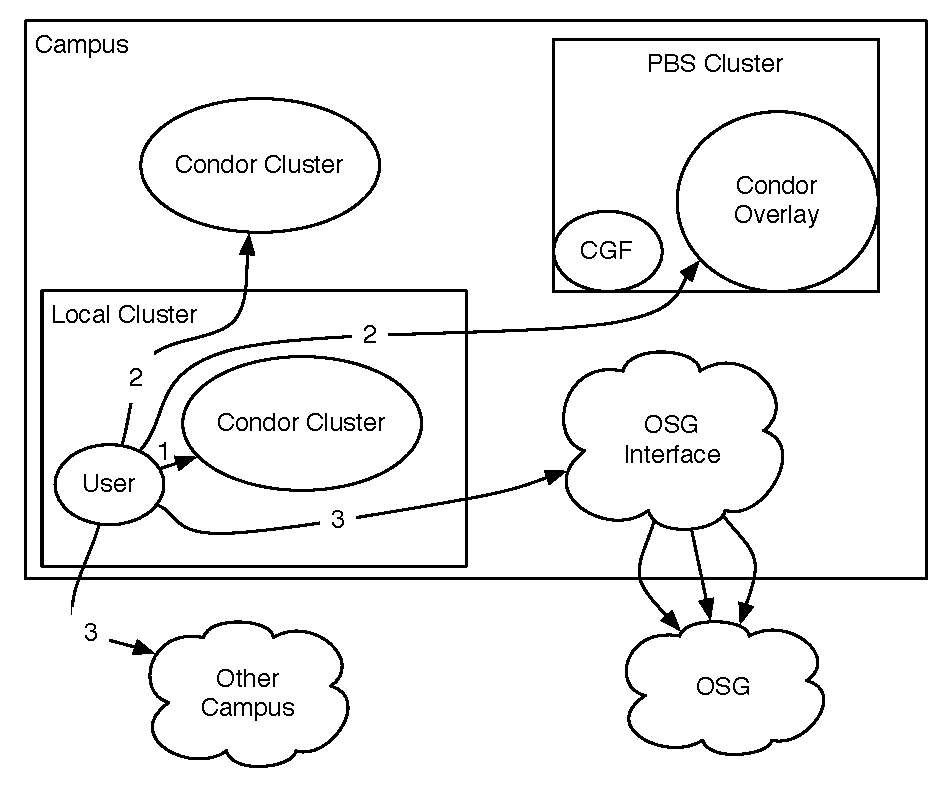
\includegraphics[scale=0.8]{images/CHEP-Campus}
\caption{The HCC Campus Grid architecture, complete with connections to other campuses and the OSG.  As each resource 
becomes fully utilized, the user's jobs will extend out to increasingly remote clusters.}
\label{fig:campusgrid}
\end{center}
\end{figure}

The full campus grid architecture with bridging is shown in Figure \ref{fig:campusgrid}.  In this campus grid, the 
user first submits jobs to the local Condor cluster (1).  If the local cluster can fulfill the user's needs, then the 
jobs will remain there.  If the local cluster is full or cannot meet the user's demand, Condor flocking will start 
submitting jobs to other campus clusters (2), either Condor or CGF-based.  If the on-campus 
resources are unable to meet the user's request, the local Condor schedd will expand its reach again (3) by looking 
outside the campus.  The jobs can also be sent to the OSG via flocking to a GlideinWMS 
frontend, which creates an overlay pool of grid resources.  In this architecture, every effort is given to find 
resources for the user (local, across campus, or externally), while maintaining the same vanilla Condor interface.






%\textbf{ Campus Factory is the heart of the operation.  It provides all throttling and logic to the submit of glidein jobs to the non-condor cluster.}











\section{Bridging Campus Grids} \label{sec:bridging}
There are two methods for expanding the campus grid described in Section \ref{sec:hcc}: through GlideinWMS to the OSG, 
or by linking campus grids through flocking.  The benefits of bridging externally are obvious - increased throughput 
for the local user's jobs.  HCC has been able to utilize over 7,000 remote job slots at a time, and has been able to 
bridge to all the campus grids discussed in Section \ref{sec:others}.  We connect to FermiGrid and GLOW through the OSG and 
to Purdue via Condor flocking.

Unlike the OSG, where the trust relationship is well-defined and common between sites, trust is established between 
campuses with flocking on a case-by-case basis.
The current model for trust is based on limited trusted hosts.  Each site publishes a list of submit and negotiator 
hosts that are trusted to submit and accept jobs, respectively.  This implicitly trusts an entire campus, while the OSG 
trust model is based on virtual organizations that may have no relationship to a physical campus or submit host.



It is important to note the ever-widening circle of resources expands from the locality of the user.  It goes from the resource 
the user knows best (and has the best support for) to the most foreign one.  This is a very natural progression, and 
each step described comes with more complexity, and new failure modes.  If the user is ever frustrated at one 
transition, he can just remain contented with the resources he has, as opposed to having to switch between ``local 
mode" and ``grid mode".  Another usability boost is that all end-user interfaces are Condor vanilla universe.  The user 
never encounters errors translated between systems (a common user frustration) and the user needs to develop expertise 
in Condor alone.





\chapter{Evaluation}
\label{sec:Evaluation}

%\section{Experimental Setup}

\section{Holland Computing Center campus grid} \label{sec:hcc}

In order to test the framework described in this paper, we created a campus grid at Nebraska.  A diagram describing the HCC campus grid is shown in Figure \ref{fig:hccgrid}.  In this diagram the user submits jobs on a central machine.  First, the jobs will attempt to run on local resources at Prairiefire and Firefly.  Next, it will branch out to the GlideinWMS interface and Purdue.

\begin{figure}[h!tb]
\begin{center}
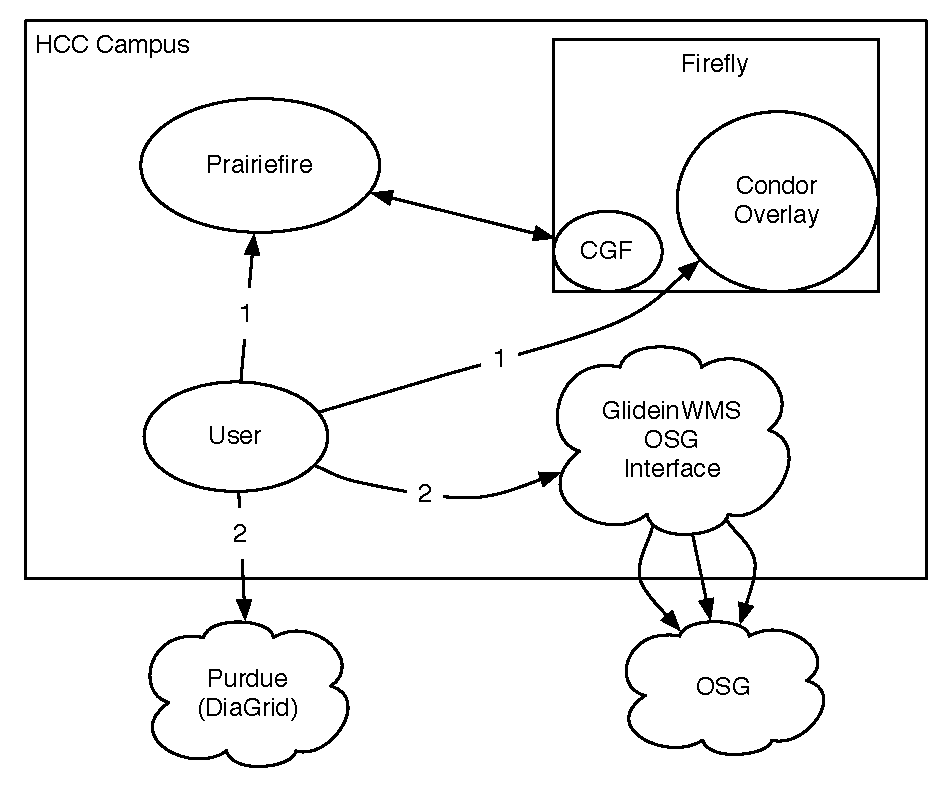
\includegraphics[scale=0.8]{images/HCC-CampusGrid-012411}
\caption{The HCC Campus Grid}
\label{fig:hccgrid}
\end{center}
\end{figure}


Like Purdue and GLOW, we have based the campus grid upon Condor.  Each resource has a Condor-based interface, giving an 
identical experience regardless of what the user considers his or her ``local" cluster.  While two of the local 
clusters run Condor as the primary batch system, one is based upon PBS.  PBS was chosen because of its superior 
scheduling of large-scale MPI jobs required for that resource.  GLOW's Condor-only approach did not fit our case, and 
Purdue's model of running multiple schedulers was rejected because we wanted a less-invasive approach and because we 
wanted more efficient scheduling.  So, for integrating our PBS cluster, we developed the Campus Grid Factory (CGF) to 
provide a Condor interface for the non-Condor clusters; this is covered in Section \ref{sec:cgf}.

To enable decentralized operation, we utilized Condor flocking \cite{epema1996worldwide} between clusters.  Condor 
flocking enables a transparent execution environment by 
imitating the interaction between submit and execute hosts when talking to remote resources.  The jobs will continue 
to be managed by the original user's submit host, but the execute hosts can be outside what is managed by the local 
Condor pool.  Furthermore, flocking can handle communication errors between remote hosts and can recover, 
providing disconnected operation when resources are unreachable.

Through Condor flocking and the CGF, we have successfully encompassed all local resources.  To provide even more value 
to HCC, jobs can also bridge to the OSG and other campus grids.  The interface to the OSG uses the GlideinWMS \cite
{sfiligoi2008glideinwms, sfiligoi2008making} frontend software, while we link to other campuses using Condor flocking 
(the same method Purdue uses to link the campuses of DiaGrid).  Unlike Condor-G, which provides a Condor interface to 
GRAM, these two methods give the same user experience as using Condor as a batch system.

All clusters on the campus grid are managed by the Holland Computing Center, therefore the trust relationship 
between the hosts are implicitly strong.  A special account is set aside on the PBS cluster for the CGF to run 
campus grid jobs.  On the Condor-managed cluster, campus grid jobs run as user \texttt{nobody} while locally-submitted 
jobs run as the submitting user.

While all resources are run by the same team, we have the ability to provide distinct user priorities per resource 
through Condor.  Further, because Condor runs {\textit inside} PBS rather than alongside it, PBS can schedule its jobs 
without interrupting Condor ones.  An administrator can prioritize jobs submitted directly from the local cluster over 
those from a remote submission, even for the same user.

Each submission host runs the Gratia accounting software to provide user accounting.  Gratia was chosen because it has 
a clean separation between remote clusters and the central database (updates are done via HTTP), ability to integrate 
new resource types easily, and its ability to integrate into the larger OSG accounting.  For integration in the OSG, 
we have extended the software to record both the submission host and the remote OSG cluster utilized.

HCC does not have a shared filesystem across all clusters, so campus grid data management is handled by Condor file 
transfer.

%\subsubsection*{Social political stuff}

%\subsubsection*{How we tested our solution}


The environment includes two local clusters, as well as an interface to the OSG and another campus grid.

\subsection{Prairiefire Cluster Setup}
Prairiefire is setup as running both Condor and PBS.  This is very similar to how Purdue uses Condor.  When a PBS arrives on a node, the Condor daemons will preempt the running job, and move to another node.  Therefore, PBS has priority access to nodes, while Condor is treated as an opportunistic user.

Condor runs on the head node of the cluster.  The head node has both a public and private interface.  Each worker node connects to the outside world through a NAT.  Since Condor must have direct communication between the submitter (possibly outside of Prairiefire) and the execute host (worker nodes), Prairiefire must run the Condor Connection Broker (CCB).  The CCB runs on the head node and negotiates connections for nodes behind the NAT to connect with the submitter.

Prairiefire is setup to allow jobs from Firefly and the GlideWMS submit machine to run.  Prairiefire's head node can also flock jobs to Firefly.  To do this, the configuration variable \texttt{FLOCK\_FROM} was set to \texttt{ff-grid.unl.edu, glidein.unl.edu} and \texttt{FLOCK\_FROM} to \texttt{ff-grid.unl.edu}.   Further, the security is setup such that jobs coming from outside of the Prairiefire pool will use the user \texttt{nobody} when running the job.  Condor uses this underprivileged account so that a rogue user can cause minimal impact to the system, and to protect other users of the system.  The security on the machine is IP based, it trusts all users from certain hosts.




\subsection{Firefly Cluster Setup}
Firefly is running the Campus Grid Factory (CGF).  It is running on the grid gatekeeper since it needs access to both the public ip and PBS submission.  Additionally, unlike the login node, the grid gatekeeper does not have a firewall.

The CGF runs as a local unprivileged user on the gatekeeper.  Condor is installed in the user's home directory and runs as the user as well.  The CGF runs as a condor job, therefore it is maintained and monitored by the Condor daemons.  Submissions to PBS are to the default user queue.

The Condor instance that runs on the gatekeeper is configured to allow flocked jobs from Prairiefire and the GlideinWMS submission node.  Also, users can submit jobs to the Condor instance, allowing them to run on Firefly or by being flocked to Prairiefire.



\subsection{GlideinWMS OSG Interface Setup}
The GldieinWMS interface is running the GlideinWMS Frontend software, as well as a Condor installation.  The Frontend periodically queries the queues of multiple machines to detect idle jobs.  When idle jobs are present, the Frontend sends a request for glideins to be submitted to the Factory.  The HCC Frontend requests glideins from the central OSG factory run at UCSD.  

Glideins are submitted to resources across the country on behalf of HCC.  When the Glidein jobs start on the remote resources, they pull condor executables from the central factory, starts them, and contacts the HCC Frontend to request jobs.


\subsection{Flocking to Purdue Setup}
Flocking to Purdue is enabled by publishing a list of collectors and schedds at Purdue and Nebraska.  This list is then inserted into the configurations of machines that will send and receive jobs.  The collector locations are placed in \texttt{FLOCK\_TO} and the schedds are specified in \texttt{FLOCK\_FROM}.

Security between the hosts are established with the \texttt{CLAIMTOBE} environment in Condor.  In this environment, Condor trusts the daemons to give accurate information on job ownership and authentication.  The security is further refined by limiting the authentication to only the Collector and Schedd hosts specified above.

In total, Purdue has 7 collectors and 6 schedds participating in the flocking.  Nebraska has 2 collectors and 3 Schedds.


\subsection{User submission}
User submission is by design very similar to submission on a dedicated Condor resource.   The user will specify the executable and where to store the stdout and stderr.  Input files are transferred per-job to the execute machine.  Condor will automatically determine output files by scanning the sandbox directory for any new files created.  The new files will be transferred back to the submitter.

Condor will only transfer files when the variables \texttt{should\_transfer\_files} and \texttt{when\_to\_transfer\_output} are set.  A typical submission file is shown in Figure \ref{fig:submission}.  In the example, Condor will transfer the executable (\texttt{/bin/hostname}) to the execute host.  Condor will return the stdout and stderr from the execute host back to the submitter.

\begin{figure}[h!t]



\lstset{
backgroundcolor=\color{white},
showspaces=false}
\begin{lstlisting}[frame=tblr]
universe = vanilla 
output = condor_out/ouptut 
error = condor_out/error 
executable = /bin/hostname 
log = test.log 
when_to_transfer_output = ON_EXIT 
should_transfer_files = YES 
queue 
\end{lstlisting}



\caption{Test test submission script} \label{fig:submission}
\end{figure}


\section{Characteristics of Campus Grid}
Here I will evaluate the HCC campus grid on the characteristics defined in Section \ref{sec:attributes}.  

\subsection{Trust relationships}
On most campuses, trust relationships are very strong.  On some campuses, a single group maintains the campus clusters.  On others, proximity of administrators have facilitated trust.

At HCC, one group administers the clusters on campus, therefore the trust relationship is strong.  The execution gateways in the campus grid restrict access by IP address.  Therefore, there is a set of trusted submission hosts.  Each host trusts each other's claimed user authentication.   Additionally, jobs running on the CGF use a valid user account rather than a un-privileged account.

When we compare this to other campus grids, we can see that the IP based filtering policy is consistent with other campuses, and less restrictive than others.  

In the Virginia Campus Grid the user uses an authentication method consistent with on-campus policies to create a token that is inconsistent with on-campus policies.  The user first authenticates with local LDAP servers, then creates a PKI certificate to interact with the on campus clusters.  The series of interactions complicates the authentication with the servers, and necessitated the creation of a separate daemon called CredEx.  The HCC policy requires only one authentication with a submit host to have access to the campus grid.

In the Oxford Campus Grid, Kerberos is used for on campus submissions, while PKI is used for external access.  This is consistent with on-campus policies.

The OSG focuses on the security of execution gateways (Compute Elements) as opposed to the security of submission hosts.  I believe this to be a mistake.  Though a compromise of a gateway can lead to access of many short lived, limited proxies.  The compromise of a submission host can give access to a long lived, unlimited proxy of a few users.  Further, since the OSG allows multiple submission hosts, and they are relatively easy to setup, there are many submission hosts.  Also, gateways are traditionally mantained by professional or knowledgable administrators, where submission hosts are usually maintained by scientists with limited knowledge of security.  Therefore, submission hosts could be compromised without knowledge of their owners, and could give access to unlimited certificates.

The GLOW and Purdue campus grids are similarly IP security based grids.  The IP based security simplifies the setup of a grid based on Condor flocking that GLOW, Purdue, and HCC use.  The IP based security protects gateway hosts by only allowing very specific submission hosts.  Further, the submission host is protected since it only submits jobs to known good hosts.

The trust relationships inside campuses are simple compared to those outside of campus.  When jobs begin flowing outside the local domain, the authentication must match that of the external entity.  In the case of HCC, jobs flow out of the grid through flocking to external campuses and to the OSG through the GlideinWMS interface.

When flocking to external campuses, the HCC grid again uses IP based security as negotiated with the campuses.  In practice, this involves publishing a list of trusted hosts on each campus.  Since campuses usually use a single authentication method for all of their machines, this creates a scenario where either a campus will trust the entirety of another campus, or not at all.  For example, HCC trusts all of Purdue's submit hosts, and therefore all of the Purdue users.  More accurately, we trust the Purdue admins to monitor the usage of their users, and to contain and contact us about possible security threats.

When jobs move the OSG, we must match the authentication methods used on the grid, PKI.  GlideinWMS simplifies this as we use a single certificate to authenticate the GlideinWMS pilot, and user jobs may not require further credentials when running.

The HCC campus grid creates a trust web inside campus composed of IP based security.  Outside of campus, it conforms to the external requirements for authentication with either a published list of trusted hosts, or an PKI certificate.

\subsection{Job Submission}
Users have the most interaction with the job submission mechanism.  Therefore, it must be simple and intuitive.  Most campuses further refine their submissions to distribute work across multiple resources.

The Virginia campus grid and the Oxford grid use globus to submit and receive jobs.  Oxford further created a resource broker to balance load among campus resources.

In the HCC, GLOW. and Purdue campuses, jobs are flocked to execute hosts inside the campus, automatically spreading out the load to available resources.  Condor takes a greedy approach to scheduling jobs, if there an empty slot, it will fill it without thinking of future submission or other resources.  Therefore, a user submits many jobs, and the first resource that it contacts has many idle slots, it will fill those slots without looking at other resources.  Though, Condor will fair share across all users of the pool.

Submission on the HCC, GLOW and Purdue grid requires only 2 more lines to the regular Condor submit file.  Additionally, all negotiation and load balancing are handled by Condor internally, therefore there is less dependency on outside sources.  


\subsection{Resource Independence}
In the OSG, resource independence is guaranteed by strict separation of resources.  This is accomplished by independent clusters having all necessary infrastructure installed locally, while only sending non-blocking information to a distributed set of central services.  This is very similar to the design of the HCC campus grid.

The HCC Campus grid installs all infrastructure to distribute jobs on the local resource.  For a Condor cluster, this is simply the existing Condor instance.  While on the PBS cluster, the CGF install is installed locally on the gatekeeper node.  Therefore, possible failures are:
\begin{itemize}
\item \textbf{Submitter failure}: The user's submission machine is taken offline only jobs submitted on this resource will be effected.  Any jobs that where currently running will be recoverable for a short time while the job lease is active.
\item \textbf{Condor cluster failure}: If the cluster becomes disconnected from the network, obs running on the cluster with remote owners will terminate after their job leases have expired.  Jobs submitted locally will continue to run on local resources, but will be unable to run on remote resources.  If the Condor instance is terminated, the locally submitted jobs will live for the lease time, then terminate.
\item \textbf{CGF installed cluster failure}:  Remotely submitted jobs will terminate after their lease has expired.  Locally submitted jobs will continue to run on local resources, including glideins previously running under PBS.  If the CGF is terminated, no more glideins will be submitted to PBS, but jobs will continue to execute on existing glideins.  Additionally, Condor will attempt to restart the CGF if it terminates abnormally.  If Condor is terminated, local jobs will execute until their job leases have expired, and glideins will shut down after receiving no new jobs.
\end{itemize}



\subsection{Accounting}

\subsection{Data Management}

\begin{itemize}
%\item   Performance metrics 
%\item   Performance parameters
%\item   Experimental design

\item Production jobs on Firefly

\end{itemize}


\subsubsection*{How our solution performed, how its performance compared to
that of other solutions mentioned in related work, and how these results show
that our solution is effective}

\begin{itemize}
%\item   Presentation and Interpretation
%\item   Why, how, and to what degree our solution is better
%\item   Why the reader should be impressed with our solution
%\item   Comments

\item
Faster job submission and start than globus.  Should be easy to show.

\item
Run at other campuses.

\item
Submit jobs between campuses.

\end{itemize}


\subsubsection*{Context and limitations of our solution as required for 
summation}
\begin{itemize}
%\item   What the results {\em do} and {\em do not} say
\item
Therefore, my solution is awesome.

\end{itemize}



\chapter{Conclusions and Future Work}
\label{sec:Conclusion}

\subsubsection*{The problem we have solved}
\begin{itemize}

%\item   The most succinct statement of the problem in the paper. Ideally one
%sentence. More realistically two or three. Remember that you simply state it
%without argument. If you have written a good paper you are simply reminding the
%reader of what they now believe and of how much they agree with you.

\item
The framework that I have described here creates a grid of clusters that can overflow to each other, and out to the other grids such as the Open Science Grid, or other campuses.  

\end{itemize}



\subsubsection*{Our solution to the problem}
\begin{itemize}

%\item    
%Again, the succinct statement that you have presented a solution

%\item   Sometimes it works well to leave it at that and not even describe your
%solution here. If you do, then again state your solution in one or two
%sentences taking the rhetorical stance that this is all obvious. If you have a
%good solution and have written an effective paper, then the reader already
%agrees with you.

\item
Combination of Condor, Glidein, and BLAHP.

\end{itemize}



\subsubsection*{Why our solution is worthwhile in some significant way}
\begin{itemize}

%\item   
%Again, a succinct restatement in just a few sentences of why your solution is
%worthwhile assuming the reader already agrees with you

\item
This solution keeps the administrator in control of priorities and access policies.  It can also follow the campus' security model.

\end{itemize}



%Why the reader should be impressed and/or pleased to have read the paper
\begin{itemize}

%\item   A few sentences about why your solution is valuable, and thus why the
%reader should be glad to have read the paper and why they should be glad you
%did this work.

\item
Provides a cookie cutter, well packaged solution for campuses to deploy a campus grid.

\end{itemize}



\subsubsection*{What we will (or could) do next}
\begin{itemize}
%\item   Improve our solution
%\item   Apply our solution to harder or more realistic versions of this problem
%\item   Apply our solution or a related solution to a related problem

\item 
Scale this solution to other universities and institutions.  Already doing this with the OSG Campus Grid Initiative.

\end{itemize}


\backmatter

\bibliographystyle{plain}
\bibliography{DerekWeitzelThesis}



\end{document}

\endinput

